\chapter{Soluciones circulares a las ecuaciones de movimiento}
\label{cap:4}
\newpage

\section{Fundamentación}

En \cite{Costa-Natario-Zilhao} se estudia cómo, bajo la condición suplementaria de Mathisson-Pirani y a partir de \eqref{eq:66}, la trayectoria para una partícula con momento angular intrínseco $S$ y modelada hasta orden dipolar en la expansión multipolar (un giróscopo) viene regida por
\begin{equation}
\cd{p^{\mu}} = -\mathbb{H}^{\mu}_{\ \nu} S^{\nu},
\end{equation}
donde se define el 4-vector de espín como $$S^{\mu} := -\frac{1}{2} \epsilon^{\mu \nu \rho \sigma} S_{\nu \rho} u_{\sigma}$$.

Si estamos en un espaciotiempo de Schwarszchild, al ser éste un espaciotiempo de Petrov tipo D, podemos esperar que existan observadores tales que $\mathbb{H}_{\mu \nu}=0$. Así, para una 4-velocidad arbitraria tenemos que las componentes no-nulas del tensor gravito-magnético de mareas \eqref{eq:51} se reducen a
\begin{align}
\mathbb{H}_{r \theta} &= \alpha u^{\phi} u^{t},\\
\mathbb{H}_{\theta t} &= -\alpha u^{\phi} u^{r},\\
\mathbb{H}_{r \phi} &= \alpha u^{\theta} u^{t},\\
\mathbb{H}_{\phi t} &= \alpha u^{\theta} u^{r},
\end{align}
donde $\alpha=3M\sin\theta /r$.

La condición $u^{\theta} = u^{\phi} = 0$ implica que $\mathbb{H}=0$, permitiendo que la única condición remanente sobre la 4-velocidad es que $u^{\mu} u_{\mu} = 1$. Esto quiere decir que un giróscopo siguiendo una trayectoria radial en un espaciotiempo de Schwarszchild no experimentará ningún efecto producto de las fuerzas de marea.

A partir de lo anterior, se puede estudiar el problema análogo pero en un contexto electromagnético, es decir, la fuerza que experimentará un dipolo magnético producto de una distribución esférica de carga total $Q$ viene determinada por
\begin{equation}
\label{eq:magforce}
\cd{p^{\mu}} = \mathtt{B}^{\ \mu}_{\nu} \mu^{\nu},
\end{equation}
donde las componentes no-nulas del tensor magnético de mareas son:
\begin{align}
\mathtt{B}_{r \theta} &= \alpha u^{\phi},\\
\mathtt{B}_{\theta r} &= 2\alpha u^{\phi},\\
\mathtt{B}_{r \phi} &= -\alpha u^{\theta},\\
\mathtt{B}_{\phi r} &= -2\alpha u^{\phi},\\
\mathtt{B}_{\theta \phi} &= \alpha u^{r},\\
\mathtt{B}_{\phi \theta} &= -\alpha u^{r},
\end{align}
y $\alpha=3Q \sin \theta /r$

Siguiendo un análisis similar, la única condición que permite hacer nulas todas las componentes del tensor magnético de mareas es $u^i=0$, es decir, cuando el dipolo magnético se encuentra en reposo respecto a la distribución esférica central.

Es interesante notar que para velocidades radiales, es decir velocidades tales que $u^{\theta} = u^{\phi} = 0$, el tensor magnético de mareas se reduce solo a su parte antisimétrica, y a partir de \eqref{eq:maxwell4} queda en evidencia que esto es producto de que un dipolo magnético en movimiento siempre experimentará un tensor de mareas no-nulo producto de los efectos de inducción magnética, lo cual nuevamente marca una gran diferencia respecto de su contraparte gravitacional.

Es posible realizar un análisis similar en el caso en que la distribución de carga $Q$ tiene un momento magnético $\mu_s$, así la fuerza que experimenta un dipolo magnético viene dada por \eqref{eq:magforce} Las componentes no-nulas del tensor de mareas en el plano equatorial son:
\begin{align}
\mathtt{B}_{r \theta} &= \alpha \left( r^2 Q u^{\phi} - 3\mu_s u^t \right),\\
\mathtt{B}_{\theta r} &= \alpha \left( 2r^2 Q u^{\phi} - 3\mu_s u^t \right),\\
\mathtt{B}_{r \phi} &= -\alpha Q r^2 u^{\theta},\\
\mathtt{B}_{\phi r} &= -2\alpha Q r^2 u^{\theta,}\\
\mathtt{B}_{t r} &= 3 \alpha \mu_s u^{\theta},\\
\mathtt{B}_{t \theta} &= 3 \alpha \mu_s u^{r},
\end{align}
donde $\alpha = 1/r^3$.

Análogamente al caso sin momento magnético $\mu_s$, no es posible anular completamente el tensor de mareas magnético, sin embargo la condición que permite anular la parte simétrica de dicho tensor viene dada por $u^r=u^{\theta}=0$ y por
\begin{equation}
\label{eq:angular-velocity-em}
\omega := \dv{\phi}{t} = 2 \frac{\mu_s}{Q r^2} = \frac{J}{Mr^2},
\end{equation}
donde $\omega$ es la velocidad angular de la órbita del dipolo, y en la última igualdad se ha usado la relación entre el momento magnético y el momento angular de la distribución.

De esta forma, para órbitas circulares tales que el dipolo tenga una velocidad angular igual a \eqref{eq:angular-velocity-em}, el tensor de mareas se reduce a su parte antisimétrica $\mathtt{B}_{\mu \nu} = \mathtt{B}_{[\mu \nu]}$, y así un dipolo magnético siguiendo una trayectoria con tales características siempre experimentará una fuerza producto del campo externo.

\begin{figure}[!ht]
\centering
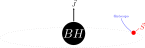
\includegraphics[scale=0.9]{images/solucion-en-kerr.pdf}
\caption[Solución helicoidal en Kerr]{Representación esquemática del sistema agujero negro-dipolo.}
\label{fig:7}
\end{figure}

Si estudiamos ahora el análogo gravitacional del problema, es decir, un giróscopo orbitando alrededor de un agujero negro rotante (ver figura \ref{fig:7}), las componentes no-nulas del tensor gravito-magnético de mareas en el plano ecuatorial son:
\begin{align}
\mathbb{H}_{r \theta} &= \alpha \left[\left(2a^2+r^2\right) u^{\phi} u^t - a\left( a^2+r^2 \right) \left( u^{\phi} \right)^2 - a\left( u^t \right)^2  \right],\\
\mathbb{H}_{r \phi} &= \alpha \left( a^2+r^2 \right) \left( au^{\phi} - u^t \right)u^{\theta},\\
\mathbb{H}_{r t} &= \alpha a \left( au^{\phi} - u^t \right)u^{\theta},\\
\mathbb{H}_{\theta \phi} &= \alpha a \left[ \left( a^2+r^2 \right) u^{\theta} - au^t \right] u^r,\\
\mathbb{H}_{\theta t} &= -\alpha \left[ \left( a^2+r^2 \right) u^{\theta} - au^t \right] u^r,\\
\mathbb{H}_{\phi \phi} &= \mathbb{H}_{tt} = -2\alpha a u^r u^{\theta}, \\
\mathbb{H}_{\phi t} &= \alpha \left( 2a^2 + r^2 \right) u^r u^{\theta},
\end{align}
donde ahora $\alpha= 3M/r^3$.

Se puede apreciar que, a diferencia del caso electromagnético, si es posible anular completamente el tensor de mareas. Las condiciones necesarias para ésto son que $u^{\theta}=0$ y  que
\begin{equation}
\label{eq:68}
\omega := \dv{\phi}{t} = \frac{a}{a^2 + r^2},
\end{equation}
donde nuevamente $\omega$ representa la velocidad angular de la órbita.

De esta forma, las ecuaciones que determinan el movimiento del giróscopo vienen dadas por 
\begin{equation}
\label{eq:69}
\cd{p^{\mu}} = 0.
\end{equation}

Esto nos lleva a la pregunta de si existen geodésicas tales que las condiciones anteriormente mencionadas sean válidas. Las más simples de estudiar son las geodésicas circulares, es decir cuando además $u^r=0$. Sin embargo podemos refutar dicha hipótesis a partir del hecho que, para geodésicas circulares, las velocidades angulares en dichas órbitas vienen determinadas por \cite{Matolcsi} 
\begin{equation}
\label{eq:angular-velocity-geodesic}
\omega_{\mathrm{geo}} = \frac{1}{a + \sqrt{\frac{r^3}{M}}}.
\end{equation}

Al igualar \eqref{eq:68} y \eqref{eq:angular-velocity-geodesic} se puede determinar que el radio de la órbita es $R=a^2/M$. Siendo éste el único radio compatible con una geodésica que satisfaga las condiciones ésta se debería encontrar dentro del horizonte de eventos, lo que nos permite demostrar que no existen geodésicas circulares tales que $\mathbb{H}_{\mu \nu}=0$

Habiendo descartado la existencia de geodésicas que satisfagan las condiciones anteriormente planteadas, una pregunta remamente es si existen soluciones, no necesariamente geodésicas, que sean soluciones a \eqref{eq:69} y cumplan dichas condiciones.

\section{Planteamiento de las ecuaciones}

Para responder esta pregunta planteada en el apartado anterior, procederemos a resolver las ecuaciones de movimiento \eqref{eq:69} y \eqref{eq:103}. 

Al estar considerando órbitas circulares, y si por simplicidad suponemos que se encuentra en el plano ecuatorial, la velocidad de un observador co-móvil con el giróscopo es $u^{\mu} = \left[ u^t,0,0,u^{\phi} \right]$.

De \eqref{eq:68}, y la condición de normalización $u^{\mu}u_{\nu} = 1$, se obtiene que la 4-velocidad del giróscopo es
\begin{equation}
\label{eq:70}
u^{\mu} = \left [ \frac{\left(a^{2} + r^{2}\right)}{r\sqrt{a^{2} - 2 m r + r^{2}}}, \quad 0, \quad 0, \quad \frac{a}{r\sqrt{a^{2} - 2 m r + r^{2}}}\right ],
\end{equation}
y, definiendo $u_{\mu} := g_{\mu \nu} u^{\nu}$, tenemos que
\begin{equation}
\label{eq:71}
u_{\mu} = \left [ \frac{1}{r}\sqrt{a^{2} - 2 m r + r^{2}}, \quad 0, \quad 0, \quad -\frac{a}{r} \sqrt{a^{2} - 2 m r + r^{2}} \right ].
\end{equation}

Por otro lado, a partir de la definición del 4-vector de espín, se pueden re-escribir las ecuaciones que determinan la evolución de éste, obteniendo que
\begin{equation}
\label{eq:72}
\cd{S^{\mu}} = -S_{\nu} \cd{u^{\nu}} u^{\mu}.
\end{equation}

Reemplazando \eqref{eq:70} y \eqref{eq:71} en \eqref{eq:69} y \eqref{eq:72} se deducen las siguientes ecuaciones de movimiento para el momentum y el espín:
\begin{align}
\dot{p}^t(s) &= -\frac{m(R^2-a^2)}{R(a^2-2mR+R^2)^{3/2}} p^R(s),\\
\nonumber
\dot{p}^r(s) &= -\frac{\sqrt{a^2-2mR+R^2}}{R^5} \left( -a^{2}m p^t(s) - a m \left(a^{2} + R^{2}\right) p^{\phi}(s) + a \left(a^{2} m - R^{3}\right) p^{\phi}(s) \right.\\
& \quad \left. + m \left(a^{2} + R^{2} \right) p^t(s) \right),\\
\dot{p}^{\theta}(s) &= 0,\\
\dot{p}^{\phi}(s) &= -\frac{a(R-m)}{R(a^2-2mR+R^2)^{3/2}} p^r(s),\\
\dot{S}^t(s) &= -\frac{a^2}{R^2 \sqrt{a^2-2mR + R^2}} S^r(s),\\
\nonumber
\dot{S}^r(s) &= -\frac{\sqrt{a^2-2mR+R^2}}{R^5} \left( - a^{2} m S^t(s) - a m \left(a^{2} + R^{2}\right) S^{\phi}(s) + a \left(a^{2} m - R^{3}\right) S^{\phi}(s) \right.\\
& \quad \left. + m \left(a^{2} + R^{2} \right) S^t(s) \right),\\
\dot{S}^{\theta}(s) &= 0,\\
\dot{S}^{\phi}(s) &= \frac{a}{R\sqrt{a^2-2mR+R^2}} S^r(s).
\end{align} 

Las cuales son dos conjuntos de 4 ecuaciones ordinarias acopladas.

\section{Soluciones}

Luego de resolver las ecuaciones analíticamente, tenemos que la forma general de la solución es, para el caso del momentum, de la forma
\begin{align}
p^t(s) &= C_1 \alpha + \beta \left( C_2 e^{s \gamma} + C_3 e^{-s \gamma} \right),\\
p^r(s) &= \delta \left( C_2 e^{s \epsilon} - C_3 e^{-s \epsilon} \right),\\
p^{\theta}(s) &= C_4,\\
p^{\phi}(s) &= C_1 + C_2 e^{s \epsilon} + C_3 e^{-s \epsilon},
\end{align}
y para el espín es de la forma
\begin{align}
S^t(s) &= C_5 \eta + \kappa \left[ C_6 \cos\left(\frac{as}{R^2} \right) + C_7 \sin\left(\frac{as}{R^2} \right) \right],\\
S^r(s) &= C_6 \left[ \tau \sin\left(\frac{as}{R^2} \right) - \sigma \cos\left(\frac{as}{R^2} \right) \right] 
+ C_7 \left[ \tau \cos\left(\frac{as}{R^2} \right) - \sigma \sin\left(\frac{as}{R^2} \right) \right],\\
S^{\theta}(s) &= C_8,\\
S^{\phi}(s) &= C_5 + C_6 \cos\left(\frac{as}{R^2} \right) + C_7 \sin\left(\frac{as}{R^2} \right),
\end{align}
donde todos los elementos con letras griegas son factores que dependen de $(a,m,R)$ y no jugarán un rol importante en el futuro. Por otro lado, los coeficientes $C_1, \dots, C_8$ son constantes de integración y pueden ser calculadas reemplazando la solución en las condiciones que debe satisfacer.

La primera condición que imponemos es el hecho que al 4-velocidad y el 4-vector de espín deben ser ortogonales. De esta forma encontramos que $C_5=0$.

De \eqref{eq:44} y \eqref{eq:42} encontramos que las soluciones para el momentum y el espín deben estar relacionadas de forma que
\begin{equation}
p^{\mu} = M u^{\mu} + \epsilon^{\mu \nu \alpha \beta} \Gamma^{\rho}_{\nu \sigma} u_{\rho} u_{\alpha} S_{\beta} u^{\sigma},
\end{equation}
al reemplazar $\mu=r$ y $\mu=\theta$ se determina que $C_2 = C_3 = C_6 = C_7 = 0$, teniendo así que la forma general de las soluciones se reduce a 
\begin{align}
\label{eq:73}
p^{\mu} &= \left[ p^{\phi} \frac{a(m+R)}{m}, 0, 0, p^{\phi} \right],\\
\label{eq:74}
S^{\mu} &= \left[ 0,0,S^{\theta},0 \right],
\end{align}
donde se han renombrado las constantes $C_1$ y $C_4$ por $p^{\phi}$ y $S^{\theta}$ respectivamente.

Finalmente, reemplazando $\mu=t$ y $\mu=\phi$ se obtiene un sistema de dos ecuaciones lineales y dos incógnitas
\begin{align}
\frac{a p^{\phi}(m+R)}{m} &= \frac{S^{\theta} a^{3}}{R^{2} \sqrt{a^{2} - 2 m R + R^{2}}} - \frac{S^{\theta} a m}{R\sqrt{a^{2} - 2 m R + R^{2}}} + \frac{a^{3} p^{\phi}}{m R} + \frac{a p^{\phi} R}{m},\\
p^{\phi} &= \frac{S^{\theta} a^{2}}{R^{2}\sqrt{a^{2} - 2 m R + R^{2}}} - \frac{S^{\theta} m}{R\sqrt{a^{2} - 2 m R + R^{2}}} + \frac{a^{2} p^{\phi}}{m R}.
\end{align}

Dicho sistema es a un sistema compatible indeterminado, es decir, admite un conjunto infinito de soluciones descritas por
\begin{equation}
\label{eq:75}
S^{\theta} = - \frac{p^{\phi}R \sqrt{a^2 - 2mR +R^2}}{m}.
\end{equation}

Reemplazando \eqref{eq:75} en \eqref{eq:73} y \eqref{eq:74} encontramos que la solución exacta a las ecuaciones puede escribirse en términos de $p^{\phi}$ como
\begin{align}
p^{\mu} &= \left[ p^{\phi} \frac{a(m+r)}{m},\quad 0,\quad 0,\quad p^{\phi} \right],\\
S^{\mu} &= \left[0,\quad 0,\quad -\frac{p^{\phi} \sqrt{a^2+r^2-2mr}}{mr},\quad 0\right],
\end{align}
o, en términos de $S^{\theta}$, como
\begin{align}
\label{eq:76}
p^{\mu} &= \left [ - \frac{S^{\theta} a \left(m + r\right)}{r \sqrt{a^{2} - 2 m r + r^{2}} }, \quad 0, \quad 0, \quad - \frac{S^{\theta} m}{r\sqrt{a^{2} - 2 m r + r^{2}}}\right ],\\
\label{eq:77}
S^{\mu} &= \left [ 0, \quad 0, \quad S^{\theta}, \quad 0\right ].
\end{align}

Es importante destacar que la masa del giróscopo puede calcularse como
\begin{equation}
\label{eq:78}
M := p^{\mu} u_{\mu} = -\frac{S^{\theta}a}{r},
\end{equation}
y en términos de $M$, la solución puede escribirse como
\begin{align}
\label{eq:86}
p^{\mu} &= \left [ \frac{M \left(m + r\right)}{\sqrt{a^{2} - 2 m r + r^{2}}}, \quad 0, \quad 0, \quad \frac{M m}{a \sqrt{a^{2} - 2 m r + r^{2}}}\right ],\\
\label{eq:87}
S^{\mu} &= \left [ 0, \quad 0, \quad - \frac{Mr}{a}, \quad 0\right ].
\end{align}

\newpage
\section{Propiedades de la solución}

De la solución podemos destacar varios puntos:
\begin{itemize}
\item[-] Los parámetros de la solución determinan una relación entre la masa y el espín del giróscopo, dicha relación nos da a entender que, por ejemplo, una vez fijado el valor del espín inmediatamente queda determinado el valor de la masa del giróscopo (o viceversa), de tal forma que se logre contrarrestar la atracción del agujero negro tal que la órbita se mantenga circular.
\item[-] La única dirección y sentido permitidos para el espín es ser antiparalelo a la rotación del agujero negro, esto es por el signo $-$ en \eqref{eq:78} que nos indica que el momento angular intrínseco del giróscopo debe ser opuesto a la rotación del agujero negro y el hecho de que la única componente no-nula para el espín es la componente $S^{\theta}$.
\end{itemize}

Es importante destacar que no es posible obtener el caso en la métrica de Schwarszchild a partir del resultado encontrado. Esto es por la suposición inicial al momento de plantear las ecuaciones de movimiento es que la velocidad angular del giróscopo es proporcional al parámetro rotacional del agujero negro, es decir $\omega \propto a$, y calcular el límite $a \rightarrow 0$ implica que $\omega = 0$, lo cual implicaría que la órbita no sería circular.

No obstante, es interesante hacer notar que si definimos la 4-fuerza sobre el giróscopo como
\begin{equation}
\label{eq:124}
F^{\mu} := M \cd{u^{\mu}} = \left[ 0, \frac{M(mR-a^2)}{R^3},0,0 \right],
\end{equation}
y si consideramos el caso asintótico, es decir $R \gg m $, entonces se puede deducir la ley de gravitación universal de Newton. Esto cumple con el principio de correspondencia puesto que al encontrarse lejos del agujero negro no hay diferencia entre un agujero negro rotante y el campo gravitacional generado por una distribución de masa. 

Además, al ser una órbita circular en donde la único agente externo acutuando sobre el giróscopo tiene solo componente radial no-nula se puede ver que el giróscopo presenta un movimiento circular uniforme, ya que presenta una velocidad angular constante, logrando identificar así que \eqref{eq:124} corresponde a la fuerza centrípeta de la órbita.

Por último, es necesario agregar que la velocidad coordenada tangencial de la órbita es
\begin{equation}
v = \omega R = \frac{aR}{a^2 + R^2},
\end{equation}
lo cual en el mismo límite asintótico se reduce a
\begin{equation}
\label{eq:79}
v \approx \frac{a}{R},
\end{equation}
y reemplazando en \eqref{eq:78} se tiene que
\begin{align}
\nonumber
R &= -\frac{S^{\theta}a}{M},\\
\nonumber
&= -\frac{S^{\theta}aR}{MR},\\
\label{eq:80}
&= -\frac{vS}{M},
\end{align}
donde $S = R S^{\theta}$ y es el módulo del espín (que coincide con el valor de la componente $z$ en un plano cartesiano).

Podemos agregar que \eqref{eq:80} representa la misma condición encontrada en \cite{Costa-Herdeiro-Natario-Zilhao} para el problema análogo en el espaciotiempo de Minkowski en coordenadas cartesianas mostrando así que la solución obtenida en \eqref{eq:86} y \eqref{eq:87} se reduce asintóticamente al caso en la métrica plana.